% 1964 全国卷第 7 题：两平面射影示意（矢量重绘）
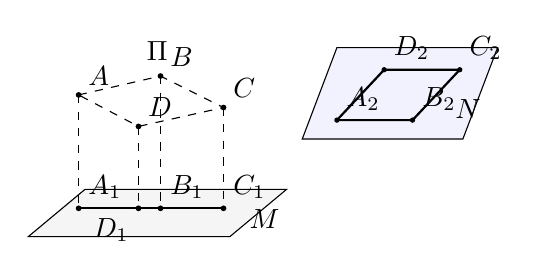
\begin{tikzpicture}[>=stealth,scale=0.8]
  % 平面 M
  \draw[fill=gray!8] (0,0) -- (3.2,0) -- (4.1,0.75) -- (0.9,0.75) -- cycle;
  \node at (3.75,0.28) {$M$};
  % 平面 N
  \draw[fill=blue!5] (4.35,1.55) -- (6.9,1.55) -- (7.45,3.0) -- (4.9,3.0) -- cycle;
  \node at (6.98,2.02) {$N$};
  % Four points in the auxiliary plane and projections to M
  \coordinate (A) at (0.8,2.25);
  \coordinate (B) at (2.1,2.55);
  \coordinate (C) at (3.1,2.05);
  \coordinate (D) at (1.75,1.75);
  \coordinate (A1) at (0.8,0.45);
  \coordinate (B1) at (2.1,0.45);
  \coordinate (C1) at (3.1,0.45);
  \coordinate (D1) at (1.75,0.45);
  \draw[dashed] (A)--(A1) (B)--(B1) (C)--(C1) (D)--(D1);
  \draw[thick] (A1)--(B1)--(C1)--(D1);
  \draw[dashed] (A)--(B)--(C)--(D)--cycle;
  \foreach \p/\name in {A/A,B/B,C/C,D/D,A1/A_1,B1/B_1,C1/C_1}
    {\fill (\p) circle (1.3pt) node[above right] {$\name$};}
  \fill (D1) circle (1.3pt) node[below left] {$D_1$};
  % Parallelogram on N
  \coordinate (A2) at (4.9,1.85);
  \coordinate (B2) at (6.1,1.85);
  \coordinate (C2) at (6.85,2.65);
  \coordinate (D2) at (5.65,2.65);
  \draw[thick] (A2)--(B2)--(C2)--(D2)--cycle;
  \foreach \p/\name in {A2/A_2,B2/B_2,C2/C_2,D2/D_2}
    {\fill (\p) circle (1.2pt) node[above right] {$\name$};}
  \node at (2.05,2.95) {$\Pi$};
\end{tikzpicture}
